% figs/actuation_modes_tikz.tex
\documentclass[tikz]{standalone}
% Common TikZ styles (standalone, robust)
\usetikzlibrary{arrows.meta,positioning,fit,calc,shapes,decorations.markings}

% 予約キー衝突や引数取りこぼしを避けるため分割宣言
\tikzset{every picture/.style={line cap=round, line join=round}}
\tikzset{box/.style={draw, rectangle, rounded corners,
  minimum width=2.2cm, minimum height=0.9cm, align=center, very thick}}
\tikzset{arrow/.style={-{Stealth}, very thick}}
\tikzset{line/.style={draw, very thick}}
\tikzset{dashedline/.style={draw, dashed, thick}}

% "node" は再定義しない。点用スタイルは独自名を使う
\tikzset{point/.style={circle, draw, minimum size=5.5mm, inner sep=0pt, thick}}

% 小さな実線ドット(Fig.2 が使う)
\tikzset{dot/.style={circle, fill, inner sep=0pt, minimum size=2.2pt}}

\tikzset{group/.style={draw, rounded corners, inner sep=5pt, thick}}
\tikzset{small/.style={font=\footnotesize}}
\tikzset{note/.style={rectangle, draw, fill=yellow!18, rounded corners,
  inner sep=2.5pt, font=\scriptsize\sffamily, thick}}
 % 共通スタイル
\begin{document}
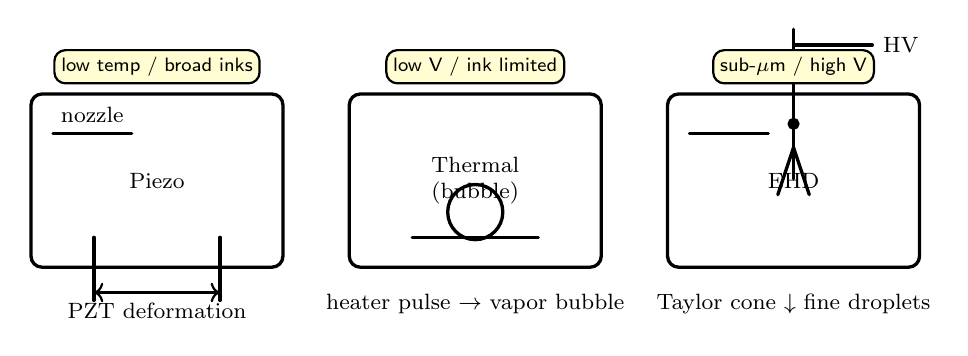
\begin{tikzpicture}[font=\footnotesize, every node/.style={align=center}]
  % 共通フレーム
  \node[box, minimum width=3.2cm, minimum height=2.2cm] (piezo)   {Piezo};
  \node[box, minimum width=3.2cm, minimum height=2.2cm, right=8mm of piezo] (thermal) {Thermal\\(bubble)};
  \node[box, minimum width=3.2cm, minimum height=2.2cm, right=8mm of thermal] (ehd) {EHD};

  % Piezo 模式図
  \draw[line] ([yshift=6mm]piezo.west)++(3mm,0) -- ++(10mm,0)
              node[above,pos=0.5]{nozzle};
  \draw[line] (piezo.south)++(-8mm,4mm) -- ++(0,-8mm);
  \draw[line] (piezo.south)++( 8mm,4mm) -- ++(0,-8mm);
  \draw[<->,thick] (piezo.south)++(-8mm,-3mm) -- ++(16mm,0)
       node[midway,below]{PZT deformation};

  % Thermal 模式図
  \draw[line] (thermal.south)++(-8mm,4mm) -- ++(16mm,0); % ヒータ面
  \draw[line] (thermal)++(0,-4mm) circle (3.5mm);        % 蒸気泡
  \node[below=2mm of thermal]{heater pulse $\rightarrow$ vapor bubble};

  % EHD 模式図
  \draw[line] ([yshift=6mm]ehd.west)++(3mm,0) -- ++(10mm,0);
  \draw[line] (ehd.north)++(0,-4mm) -- ++(0,12mm);
  \draw[fill=black] (ehd.north)++(0,-4mm) circle (0.7mm); % ノズル先端
  \draw[line] (ehd.north)++(0,6mm) -- ++(10mm,0) node[right]{HV};
  \draw[line] (ehd.north)++(0,-4mm) -- ++(0,-7mm);        % テイラーコーン
  \draw[line] (ehd.north)++(0,-7mm) -- ++(2mm,-6mm);
  \draw[line] (ehd.north)++(0,-7mm) -- ++(-2mm,-6mm);
  \node[below=2mm of ehd]{Taylor cone $\downarrow$ fine droplets};

  % タグ
  \node[note, above=1mm of piezo]   {low temp / broad inks};
  \node[note, above=1mm of thermal] {low V / ink limited};
  \node[note, above=1mm of ehd]     {sub-$\mu$m / high V};
\end{tikzpicture}
\end{document}
